
\begin{figure}
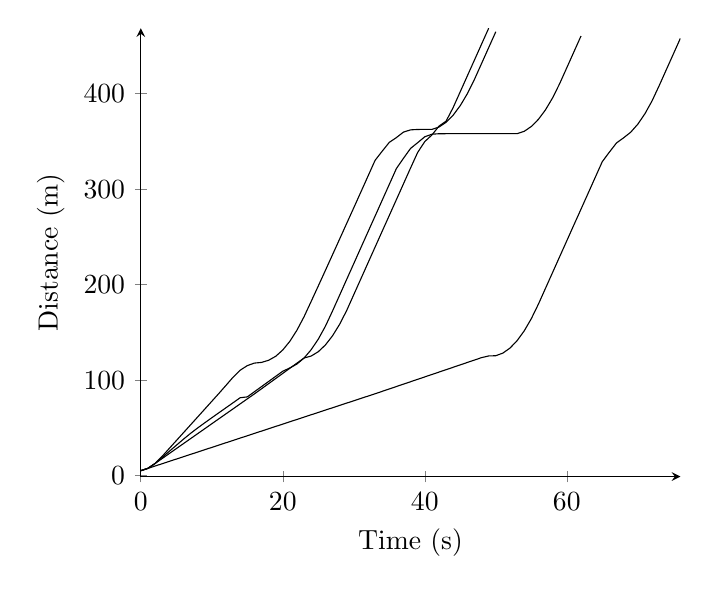
\begin{tikzpicture}
\begin{axis}[
legend style={anchor=west},
axis x line=bottom,
axis y line=left,
ymin=-1,
xlabel=Time (s),
ylabel=Distance (m),
]
\addplot[] coordinates {
(0, 5.1)
(1, 7.6)
(2, 12.6)
(3, 18.9664764928)
(4, 25.3332336511)
(5, 31.700321053)
(6, 38.0678007069)
(7, 44.1729173655)
(8, 49.8267399426)
(9, 55.25095355)
(10, 60.5637171987)
(11, 65.8239974249)
(12, 71.0602827234)
(13, 76.2862250338)
(14, 81.5703501329)
(15, 82.4483933522)
(16, 87.811906582)
(17, 93.1877672112)
(18, 98.570032102)
(19, 103.956345526)
(20, 109.326505561)
(21, 112.779004912)
(22, 116.899818957)
(23, 123.147404791)
(24, 131.894990624)
(25, 142.912472055)
(26, 156.429953486)
(27, 172.299201181)
(28, 188.899201181)
(29, 205.499201181)
(30, 222.099201181)
(31, 238.699201181)
(32, 255.299201181)
(33, 271.799201181)
(34, 288.399201181)
(35, 304.999201181)
(36, 321.599201181)
(37, 332.35676783)
(38, 342.723770794)
(39, 348.701865404)
(40, 354.904226452)
(41, 357.533785107)
(42, 358.084707081)
(43, 358.109946913)
(44, 358.109946913)
(45, 358.109946913)
(46, 358.109946913)
(47, 358.109946913)
(48, 358.109946913)
(49, 358.109946913)
(50, 358.109946913)
(51, 358.109946913)
(52, 358.109946913)
(53, 358.109946913)
(54, 360.609946913)
(55, 365.609946913)
(56, 373.109946913)
(57, 383.109946913)
(58, 395.609946913)
(59, 410.609946913)
(60, 427.209946913)
(61, 443.809946913)
(62, 460.409946913)
};
\addplot[] coordinates {
(0, 5.1)
(1, 7.6)
(2, 12.6)
(3, 17.8089879254)
(4, 23.0181600437)
(5, 28.2275422387)
(6, 33.4371654916)
(7, 38.6470672024)
(8, 43.8572929472)
(9, 49.0678988477)
(10, 54.2789548168)
(11, 59.490549087)
(12, 64.7027946549)
(13, 69.9158386643)
(14, 75.1298764297)
(15, 80.3451730339)
(16, 85.5620977864)
(17, 90.8971816382)
(18, 96.2829521364)
(19, 101.669179429)
(20, 107.056090337)
(21, 112.444096715)
(22, 117.834043217)
(23, 123.189723795)
(24, 125.23231756)
(25, 129.774911324)
(26, 136.817505088)
(27, 146.360098852)
(28, 158.402692617)
(29, 172.945286381)
(30, 189.545286381)
(31, 206.145286381)
(32, 222.745286381)
(33, 239.345286381)
(34, 255.945286381)
(35, 272.445286381)
(36, 289.045286381)
(37, 305.645286381)
(38, 322.245286381)
(39, 338.524796327)
(40, 349.874794715)
(41, 356.713114832)
(42, 366.051434949)
(43, 371.239755065)
(44, 385.578075182)
(45, 402.178075182)
(46, 418.778075182)
(47, 435.378075182)
(48, 451.978075182)
(49, 468.578075182)
};
\addplot[] coordinates {
(0, 5.1)
(1, 7.54190883705)
(2, 9.9838500455)
(3, 12.4258255054)
(4, 14.8678372455)
(5, 17.309887458)
(6, 19.7519785159)
(7, 22.1941129916)
(8, 24.6362936783)
(9, 27.0785236145)
(10, 29.5208061118)
(11, 31.9631447856)
(12, 34.4055435915)
(13, 36.8480068661)
(14, 39.2905393739)
(15, 41.733146362)
(16, 44.1758336225)
(17, 46.6186075656)
(18, 49.0614753043)
(19, 51.5044447539)
(20, 53.9475247485)
(21, 56.3907251789)
(22, 58.834057156)
(23, 61.2775332054)
(24, 63.721167501)
(25, 66.1649761464)
(26, 68.6089775163)
(27, 71.0531926733)
(28, 73.4976458808)
(29, 75.9423652384)
(30, 78.3873834757)
(31, 80.8327389533)
(32, 83.2784769378)
(33, 85.7402681571)
(34, 88.2436946102)
(35, 90.7659186044)
(36, 93.2882159343)
(37, 95.8105994658)
(38, 98.3330853019)
(39, 100.855693884)
(40, 103.378451588)
(41, 105.901393088)
(42, 108.42456499)
(43, 110.948031606)
(44, 113.47188458)
(45, 115.996259881)
(46, 118.521370109)
(47, 121.047572496)
(48, 123.575534949)
(49, 125.324959483)
(50, 125.574798377)
(51, 128.324637271)
(52, 133.574476165)
(53, 141.324315059)
(54, 151.574153953)
(55, 164.323992847)
(56, 179.573831741)
(57, 196.173831741)
(58, 212.773831741)
(59, 229.373831741)
(60, 245.973831741)
(61, 262.573831741)
(62, 279.073831741)
(63, 295.673831741)
(64, 312.273831741)
(65, 328.873831741)
(66, 338.820345134)
(67, 348.435589557)
(68, 353.76929704)
(69, 359.669231305)
(70, 368.069165571)
(71, 378.969099836)
(72, 392.369034101)
(73, 408.268968366)
(74, 424.868968366)
(75, 441.468968366)
(76, 458.068968366)
};
\addplot[] coordinates {
(0, 5.1)
(1, 7.6)
(2, 12.6)
(3, 20.1)
(4, 28.3384905751)
(5, 36.5775710795)
(6, 44.8173939803)
(7, 53.0581693688)
(8, 61.3001951102)
(9, 69.5439082112)
(10, 77.7899772328)
(11, 86.0394801664)
(12, 94.5079906685)
(13, 103.030046099)
(14, 110.370652547)
(15, 115.186154622)
(16, 117.845941477)
(17, 118.538347977)
(18, 120.79626935)
(19, 124.935896936)
(20, 131.575524522)
(21, 140.715152108)
(22, 152.354779694)
(23, 166.49440728)
(24, 182.469159771)
(25, 198.613972191)
(26, 214.881773342)
(27, 231.23890541)
(28, 247.66112139)
(29, 264.130860546)
(30, 280.535355826)
(31, 297.065299556)
(32, 313.613892411)
(33, 330.213892411)
(34, 339.762715829)
(35, 349.011565296)
(36, 354.036138596)
(37, 359.800760853)
(38, 362.121269838)
(39, 362.554368776)
(40, 362.569979692)
(41, 362.569979692)
(42, 365.069979692)
(43, 370.069979692)
(44, 377.569979692)
(45, 387.569979692)
(46, 400.069979692)
(47, 415.069979692)
(48, 431.669979692)
(49, 448.269979692)
(50, 464.869979692)
};

\end{axis}
\end{tikzpicture}
\label{tik:100:19_O, 19_O.-60, 17_N, 15_S, 15_S.-30, 14_O}
\caption{100 percent diving with GSC on route $19_O, 19_O.-60, 17_N, 15_S, 15_S.-30, 14_O$}
\end{figure}
